
\documentclass{llncs}
\usepackage{makeidx}  % allows for indexgeneration
\usepackage{acronym}
\usepackage[numbers]{natbib}
\bibliographystyle{splncs03} 
%\bibliographystyle{splncsnat} 
%\bibliographystyle{IEEEtran}


\usepackage[hyphens]{url}
\usepackage{nameref}
\usepackage{hyperref}
\usepackage[USenglish]{babel}
\usepackage[T1]{fontenc}
\usepackage{amsmath}
\usepackage{amssymb}
\usepackage{pslatex}
%

\DeclareMathOperator{\tr}{tr}
\DeclareMathOperator{\argmax}{argmax}
\DeclareMathOperator{\argmin}{argmin}
\DeclareMathOperator{\diag}{diag}
\DeclareMathOperator{\dist}{dist}
\DeclareMathOperator{\const}{Const.}

%
%\tableofcontents
%
\mainmatter              % start of the contributions
%

\begin{document}

\title{Simultaneous segmentation and distortion correction on diffusion weighted MR using shape priors}
%%
\titlerunning{Segmentation & EPI correction on DWI}  % abbreviated title (for running head)
%                                     also used for the TOC unless
%                                     \toctitle is used
%
\author{Oscar Esteban\inst{1,2} \and Alessandro Daducci \inst{2} \and
        Jean-Philippe Thiran \inst{2} \and Andr\'es Santos \inst{1} \and
        Dominique Zosso \inst{2,3}}
%
\authorrunning{Oscar Esteban et al.} % abbreviated author list (for running head)

\institute{Biomedical Image Technologies (BIT),
ETSI Telecomunicaci\'on - Universidad Polit\'ecnica de Madrid
and CIBER-BBN, \\
Av. Complutense 30, E-28040 Madrid, Spain\\
\email{oscar.esteban@upm.es},\\
% WWW home page:
%\texttt{http://users/\homedir iekeland/web/welcome.html}
\and
Signal Processing Laboratory (LTS5),
\'Ecole Polytechnique F\'ed\'erale de Lausanne (EPFL)\\
EPFL STI IEL LTS5, Station 11, CH-1015 Lausanne, Switzerland
\and
Department of Mathematics, University of California, Los Angeles (UCLA)\\
520 Portola Plaza, Box 951555, Los Angeles, CA 90095-1555, U.S.A.
}


\maketitle              % typeset the title of the contribution


\acrodef{dwi}[DWI]{Diffusion Weighted Imaging}
\acrodef{dti}[DTI]{Diffusion Tensor Imaging}
\acrodef{mr}[MR]{Magnetic Resonance}
\acrodef{mri}[MRI]{Magnetic Resonance Imaging}
\acrodef{csf}[CSF]{cerebrospinal fluid}
\acrodef{wm}[WM]{White Matter}
\acrodef{gm}[GM]{Grey Matter}
\acrodef{epi}[EPI]{echo-planar imaging}
\acrodef{fa}[FA]{fractional anisotropy}
\acrodef{md}[MD]{mean diffusivity}
\acrodef{acwe}[ACWE]{Active Contours without edges}


\begin{abstract}
Connectomics is the study of fiber connections in the brain. High-quality reconstructions of the connectome from diffusion weighted MR acquisitions require a precise delineation of pial and grey-matter-white-matter interfaces. Furthermore, to enable significant group studies, these surfaces must be located and parcellated consistently across subjects. Precise segmentation and parcellation are readily available on anatomical images, such as T1-weighted MRI. Diffusion weighted images (DWI), however, typically have drastically lower resolution and exhibit more important distortions. Here, we propose a joint segmentation-registration framework that exploits the detailed and consistent anatomy extracted from anatomical MRI as strong shape-prior for DW segmentation. We use the Mumford-Shah (or active contours without edges) model to look for a regular deformation field that optimally maps the shape prior on the multivariate features in diffusion space. Preliminary results on synthetic images and simluated DWI confirm the effectiveness of our approach.
%\dots
\keywords{diffusion weighted imaging, connectomics, echo planar imaging, magnetic resonance, segmentation, registration, distortion correction}
\end{abstract}

\section{Introduction}
\label{sec:introduction}
%
\Gls{dwi} is a widely used family of \gls{mr} techniques
\citep{sundgren_diffusion_2004} which recently has accounted for a growing
interest in its application to whole-brain structural connectivity analysis.
This emerging field, coined in 2005 as \emph{\gls{mr} Connectomics}
\citep{hagmann_diffusion_2005,sporns_human_2005}, currently includes a
large amount of imaging techniques for acquisition, processing, and analysis
specifically tuned for \gls{dwi} data.

The whole-brain connectivity analysis has given rise to some challenges
towards reliable structural information about the neuronal tracts 
from \gls{dwi} \cite{johansen-berg_using_2009,jones_white_2012}. 
The earlier stages of these processing pipelines generally include 
two necessary steps, brain tissue segmentation on the diffusion space 
and the correction of geometrical distortions inherent to the acquisition 
sequence \citep{hagmann_mr_2012}.

In this work, we will refer as brain tissue segmentation to the precise
delineation of the \gls{csf}-\gls{gm} and \gls{gm}-\gls{wm} interface surfaces.
This segmentation is a processing step on which strongly rely further
tasks. An accurate brain tissue segmentation is required
to filter the fiber bundles obtained with \gls{dwi} tractography. 
This requirement is usually solved in practice by plainly thresholding the 
\gls{fa}, a well-known scalar map derived from \gls{dwi} which depicts 
the isotropy of water diffusion inside the brain. Also,
it is necessary to locate the intersections of fiber bundles and \gls{gm}.
Moreover, a precise location of the \gls{gm}-\gls{wm} surface is also essential 
to finally achieve a consistent parcellisation of the cortex 
to represent the nodes of the output network. This parcellisation 
is generally defined in a high-resolution and better understood structural 
\gls{mri} of the same 
subject (e.g. \gls{t1} and/or \gls{t2} weighted acquisitions). Even though
some efforts have addressed the study of the robustness of tractography with
respect to intra-subject variability \cite{heiervang_between_2006,
wakana_reproducibility_2007}, these results are restricted to certain regions 
of the brain, only. Therefore, robust and precise segmentation methods are 
required in the whole-brain application. The problem is challenging due to
the much lower resolution of \gls{dwi} (typically around 
$2.5\times2.5\times2.5mm^3.$) compared to structural \gls{mri}, and the
existence of geometrical distortions.

\gls{dwi} data are usually acquired with \gls{epi} sequences 
as they allow for very fast acquisitions but they are known to 
suffer from geometrical distortions due to local field inhomogeneities. 
These artifacts happen along the phase-encoding direction, and are most 
appreciable in the front part of the brain for the strong air/tissue 
interface around the frontal sinuses. Some methodologies have
been developed and generically named as \emph{\gls{epi}-unwarp} techniques
\cite{holland_efficient_2010,hsu_correction_2009,jezzard_characterization_2005,
reber_correction_2005}. These methods usually 
require the extra acquisition of the magnitude and phase of
the field (``field-mapping''), a condition which is not always met. Some other 
methodologies do not make use of the field-mapping, compensating the distortion
with non-linear registration from structural \gls{mri} or other means
\citep{andersson_modeling_2001}. To our knowledge, there exists no study
on the impact of the \gls{epi} distortion on the variability of tractography
results. 

Therefore, the problems of precise segmentation in \gls{dwi}-space and the 
spatial mapping between these contours and the corresponding surfaces in 
anatomical images bear significant redundancy. Once the spatial relationship 
between \gls{t1} and \gls{dwi} space is established, the contours which are 
readily available in \gls{t1} space can simply be projected on to the 
\gls{dwi}-data. Conversely, if a precise delineation in \gls{dwi}-space 
was achieved, the spatial mapping with \gls{t1}-space could be derived 
from one-to-one correspondences on the contours. However, neither segmentation 
nor registration can be performed flawlessly, if considered independently. 
The significant benefits of exploiting the anatomical \gls{mri} when 
segmenting the \gls{dwi} data have been demonstrated \cite{zollei_improved_2010}, 
justifying the use of the shape prior information. 

We suggest clustering the current methodologies of template-based segmentation 
methods into three groups. The first group typically adds a shape prior term to 
the energy functional of an evolving active contour~\citep{Bresson2006a,Chan2005,
Chen2002,Cremers2006,Gastaud2004,Paragios2003,Vemuri2003a,Yezzi2003a}.
These methods generally have a explicit description of the expected relative boundary 
locations of the object to be delineated, and some even model the statistical deviations
from this average shape. Closely related to this group are atlas-based segmentation
methods \citep{Gorthi2011,Gorthi2009,Pohl2005,Pohl2006,Wang2006}, where the prior 
imposes consistent voxel-based classification of contiguous regions. Here, the 
presence of more structures than one unique \gls{roi} helps aligning the target image 
with the atlas in a hierarchical fashion. Finally, the third group generalizes 
the atlas to actual images, and the contour is to segment simultaneously two 
different target images, related by a spatial transform to be co-estimated~\citep{Wyatt2003,
Yezzi2003}.

In this paper we propose a novel registration framework to simultaneously
solving the segmentation and distortion challenges, by exploiting as strong 
shape-prior the detailed morphology extracted from high-resolution anatomical 
\gls{mri}. Indeed, hereafter we assume this segmentation problem in anatomical 
images as a solved by widely used available procedures.
Moreover, the shape prior is of very ``strong'' nature, since it is specific to 
the particular subject. Also, after global alignment using existing approaches, 
the remaining spatial deformation between anatomical and diffusion space is 
due to \gls{epi} distortions. Finally, we need to establish precise spatial 
correspondence between the surfaces in both spaces, including the tangential 
direction for parcellation. Therefore, we can reduce the problem to finding 
the differences of spatial distortion in between anatomical and \gls{dw} space.
We thus reformulate the segmentation problem as an inverse problem, where we 
seek for an underlying deformation field (the distortion) mapping 
from the structural space into the diffusion space, such that the structural 
contours segment optimally the \gls{dwi} data. In the process, the one-to-one 
correspondence between the contours in both spaces is guaranteed, and projection 
of parcellisation to \gls{dw} space is implicit and consistent.

We test our proposed joint segmentation-registration model on two different 
synthetic examples. The first example is a scalar sulcus model, where the 
\gls{csf}-\gls{gm} boundary particularly suffers from \gls{pve} and can only be 
segmented correctly thanks to the shape prior and its coupling with the inner, 
\gls{gm}-\gls{wm} boundary through the imposed deformation field regularity. 
The second case deals with more realistic \gls{dwi} data stemming from 
phantom simulations of a simplistic brain data. Again, we show that the 
proposed model successfully segments the \gls{dwi} data based on two derived 
scalar features, namely \gls{fa} and \gls{md}, while establishing an estimate 
of the dense distortion field.

The rest of this paper is organized as follows. First, in \autoref{sec:methods}
we introduce our proposed model for joint multivariate segmentation-registration.
Then we provide a more detailed description of the data and experimental setup in
\autoref{sec:experiments}. We present results in \autoref{sec:results} and conclude 
in \autoref{sec:conclusion}.

\section{Methods}
\label{sec:methods}
%
\subsection{Simulated datasets}
%
As described in \autoref{sec:introduction}, the general situation in
the connectivity pipelines consists on having 
a reliable segmentation obtained from the high resolution \ac{t1} 
reference image. Therefore, a precise location of the tissue interfaces
of interest is available in a reference space. Given that there is no 
interest on the anatomical reference segmentation,
we directly obtained the shape priors from the models. \\

On the other hand, the target \ac{dwi} data is characterized by its
low resolution (typically around $2.2x2.2x3mm^3$). Depending on the
posterior reconstruction methodology and the angular resolution
intended, the \ac{dwi} raw data has to be processed in order to
extract the information in a manageable manner. Particularly, we
will use the \ac{fa} and \ac{md} maps for convenience.
Whereas \ac{fa} describes the \emph{shape} of diffusion, 
the \ac{md} depicts the \emph{manitude} of the process. 
There exist two main reasons to justify their choice. 
First, they are well-understood and standardized in clinical routine.
Second, together they contain most of the information that is
usually extracted from the \ac{dwi}-derived scalar maps. \\

In order that demonstrating the functionality of the proposed
methodology and characterize its possibilities, we developed two
synthetic models and simulated their corresponding \ac{dwi}
raw signal as described in \citep{tuch_q-ball_2004}. 
(HERE WE NEED A GOOD DESCRIPTION OF THE DATA, directions, resolution, etc)
. The first model consists of several spherical shapes emulating
the different brain tissues (see \autoref{fig:fa}, first row). 
The second model is based on the BrainWeb dataset.
We reconstructed the \ac{dwi} signal with standard procedures to approximate the
environment to the real one at maximum. \\

\subsection{\acl{acwe}-like variational segmentation model}
%
Let us denote $\{c_i\}_{i=1..N_c}$ the nodes of a shape prior surface. In
our application, a precise \ac{wm}-\ac{gm} interface extracted from a
high-resolution reference volume. All the formulations can be naturally
extended to include more shape priors. On the other hand, we have a 
number of \ac{dwi}-derived features at each
voxel of the volume. Let us denote by $x$ the voxel and 
$f(x) = [ f_1, f_2, \ldots, f_N]^T(x)$ its associated feature vector.\\
%
The transformation from reference into \ac{dwi} coordinate space is 
achieved through a dense deformation field $u(x)$, such that:
%
\begin{equation}
c_i' = T\{c_i\} = c_i + u(c_i)
\end{equation}
% 
Since the nodes of the anatomical surfaces might lay off-grid, it is 
required to derive $u(x)$ from a discrete set of parameters $\{u_k\}_{k=1..K}$.
Densification is achieved through a set of associated basis functions 
$\Psi_k$ (e.g. rbf, interpolation splines):
%
\begin{equation}
u(x) = \sum_k \Psi_k(x) u_k
\end{equation}
%
Consequently, the transformation writes
%
\begin{equation}
\label{eq:transformation}
c_i' = T\{c_i\} = c_i + u(c_i) = c_i + \sum_k \Psi_k(c_i)u_k
\end{equation} 
%
% Comment: maybe this is not for IPMI 2013.
%Note that, since $c_i$ remains constant in the DW segmentation process,
%the values of $\Psi_k(c_i)$ can be precomputed. Also, provided compact 
%support of the basis functions, the system remains relatively sparse.\\
%
Based on the current estimate of the distortion $u$, we can compute 
``expected samples'' within the shape prior projected into the \ac{dwi}.
Thus, we now estimate region descriptors of the \ac{dwi} features 
$f(x)$ of the regions defined by the priors in \ac{dwi} space.
%
Using Gaussian distributions as region descriptors, we propose an
\ac{acwe}-like, piece-wise constant, variational image segmentation
model (where the unknown is the deformation field)
\cite{chan_active_2001}:
\begin{equation}
\label{eq:gaussian_energy}
E(u)= \sum_{\forall{R}} \int_{\Omega_R} (f-\mu_R)^T\Sigma_R^{-1}(f-\mu_R) dx
\end{equation}
where $R$ indexes the existing regions and the integral domains
depend on the deformation field $u$. Note
that minimizing this energy, $\argmin_u\{E\}$, yields the \ac{map} 
estimate of a piece-wise smooth image model affected by Gaussian 
additive noise. This inverse problem is ill-posed
\cite{bertero_ill-posed_1988,hadamard_sur_1902}.
In order to account for deformation field regularity and to render the 
problem well-posed, we include limiting and regularization terms into 
the energy functional \cite{morozov_linear_1975,tichonov_solution_1963}:
%
\begin{align}
\label{eq:complete_energy}
E(u) &= \sum_{\forall{R}} \lbrace \int_{\Omega_R} (f-\mu_R)^T\Sigma_R^{-1}(f-\mu_R) dx \rbrace \nonumber \\
&\quad + \alpha \int  \|u\|^2 dx + \beta \int \left( \|\nabla u_x\|^2 + \|\nabla u_y\|^2 + \|\nabla u_z\|^2\right) dx
\end{align}
%
These regularity terms ensure that the segmenting contours in 
\ac{dwi} space are still close to their native shape. The model
easily allows to incorporate inhomogeneous and anisotropic 
regularization \cite{nagel_investigation_1986} to better regularize
the \ac{epi} distortion. \\
%

At each iteration, we update the distortion along the steepest 
energy descent. This gradient descent step can be efficiently 
tackled by discretizing the time in a forward Euler scheme, 
and making the right hand side semi-implicit in the 
regularization terms:
%
\begin{align}
\frac{u^{t+1}-u^t}{\tau} &= - \sum_{i=1}^{N_c} \left[ \Delta E(f(c_i'))  \hat{n}_{c_i'} \Psi_{c_i}(x) \right] -\alpha u^{t+1} + \beta\Delta u^{t+1}
\end{align}
%
where the data terms remain functions of the current estimate 
$u^t$, thus $c_i' = c_i'(u^t)$. For simplicity on notation, we 
restricted the number of priors to only 1. We also defined 
$\Delta E(f(c_i')) = E_{out}(f(c_i')) - E_{in}(f(c_i'))$, 
and $E_R(f) = \sqrt{(f-\mu_R)^T\Sigma_R^{-1}(f-\mu_R)}$.
We applied a spectral approach to solve this implicit scheme:
%
\begin{equation}
u^{t+1} = \mathcal{F}^{-1}\left\{ \frac{\mathcal{F}\{u^t/\tau
- \sum_{i=1}^{N_c} \left[ \Delta E(f(c_i')) \hat{n}_{c_i'} \Psi_{c_i}(x) \right]  \}}{\mathcal{F}\{(1/\tau+\alpha)\mathcal{I}-\beta\Delta\}} \right\}
\end{equation}
%

\subsection{Experiment}
%
For both models, we created manually a sound distortion visually similar
to real \ac{epi} distortions. We interpolated the distortion to a 
dense deformation field, necessary for warping the raw \ac{dwi} simulated
data. Once the signal was deformed, we proceeded to reconstruct the
\ac{dti} and subsequently obtained the scalars of interest (\ac{fa}, \ac{md}) and estimated their parameters on the model.\\

We evaluate the performance of our methodology to estimate the deformation
field and compare it to the original synthetic deformation field applied to the data.


\section{Results and discussion}
\label{sec:results}

\subsection{Synthetic gray-scale data}
The proposed method solved precisely the specific challenge
created by the model. A severe distortion of the model is
artificially created adding complexity to the problem of
partial voluming in the outer contour of the sulcus.
\autoref{fig:sulcusmodel_result} provides visual assessment
for this result. With 16x16x16 control points, 
computation time for this model was around
10 minutes in a {\color{red}{(specific machine details)}}.
\begin{figure}
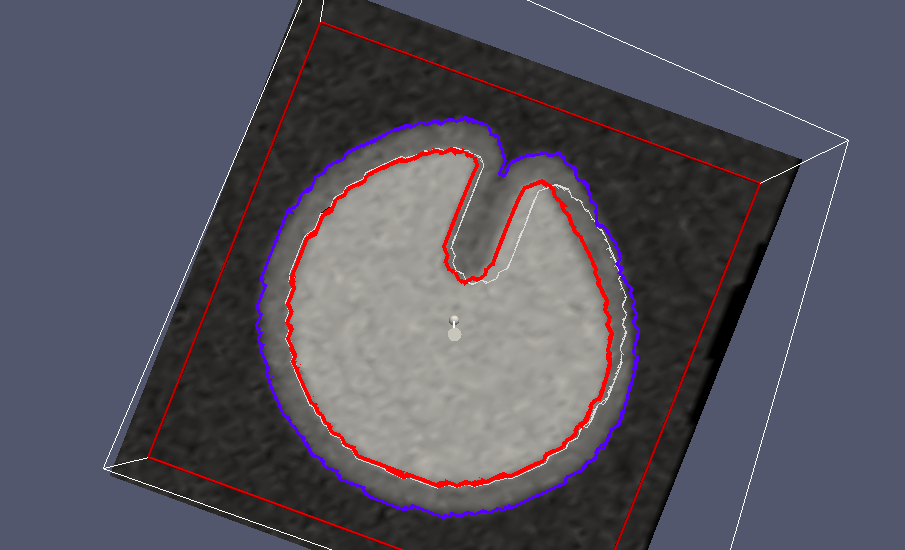
\includegraphics[width=1.0\textwidth]{model2result}
\caption{Result of the segmentation performance on the first
model. In red and blue colors the obtained \ac{wm}/\ac{gm} 
and \ac{gm}/\ac{csf} contours for the deformed image, respectively.
In white color, the initial shape priors for the \ac{wm}/\ac{gm}
interface.
{\color{red}{This figure is to be replaced by the real result,
this is a proof of concept of registration that does not solve
the pv problem. The current figure also removes the outer prior}}}
\label{fig:sulcusmodel_result}
\end{figure}


\subsection{Simulated diffusion data}
%
The proposed method successfully reverted the synthetic distortion
field we applied to the data. With 16x16x16 control points, the
displacements field is dense enough to correctly represent the
synthetic field. Second row in \autoref{fig:fa} shows the fitted
contours obtained by using the original surfaces of the model
as shape priors, with a constant translation of (5.0mm,10mm.,-5.0mm)
to illustrate briefly the extent of the capture range of the algorithm.
Computation time in this case was around 4 minutes in the previously
described platform. \\
%

\begin{figure}
\begin{tabular}{ccccc}
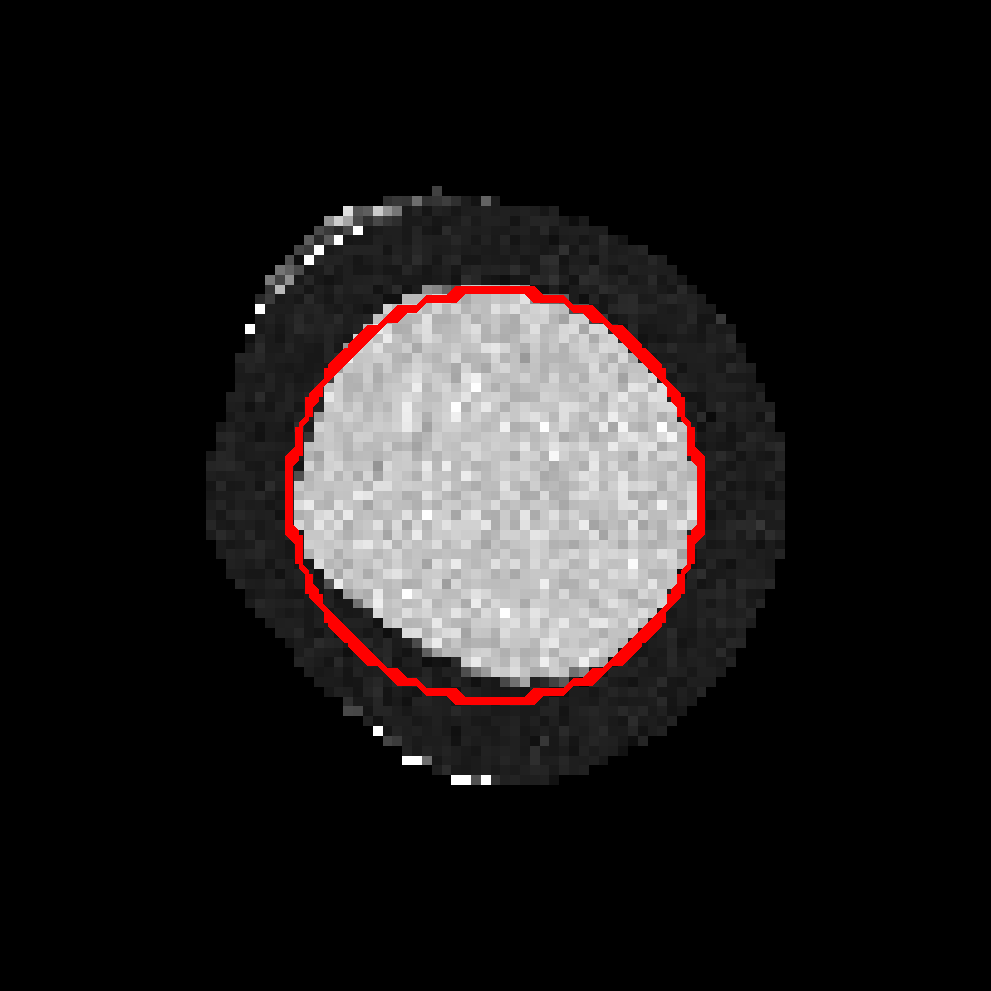
\includegraphics[width=0.19\textwidth]{model1result_b_1} &
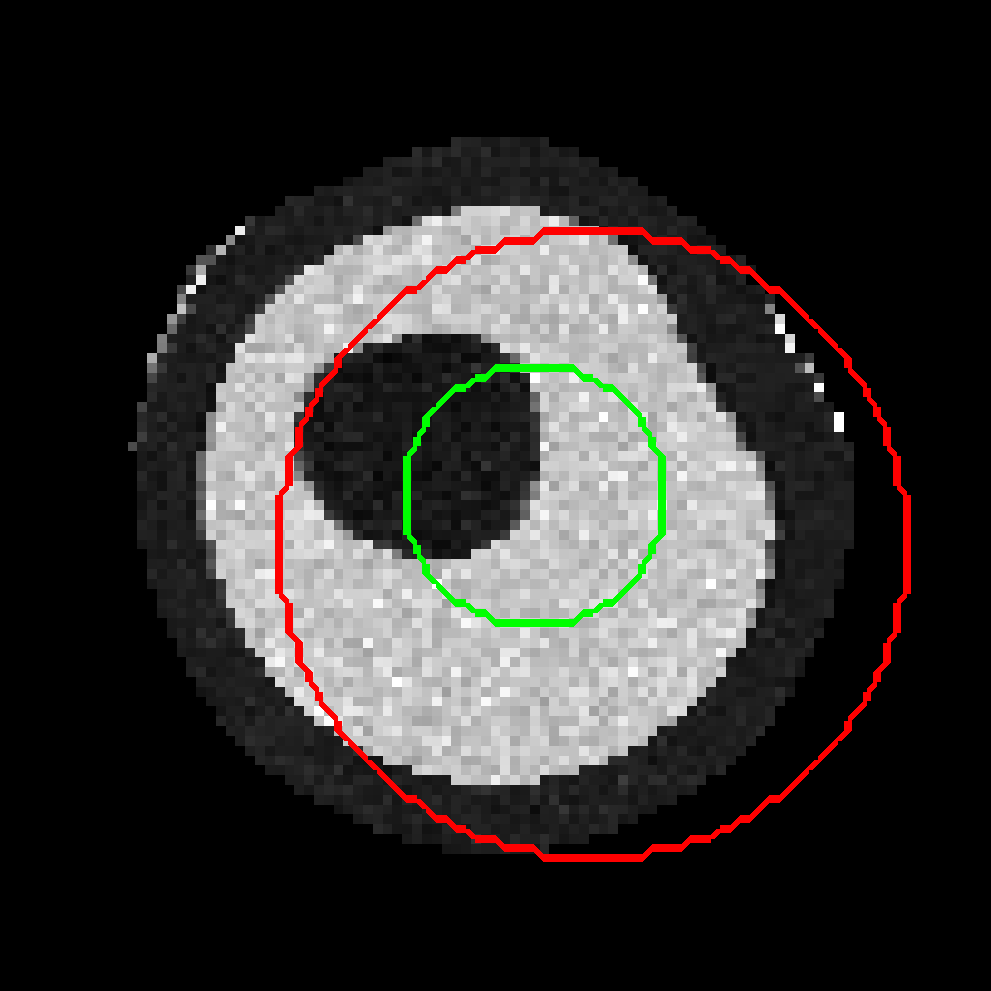
\includegraphics[width=0.19\textwidth]{model1result_b_2} &
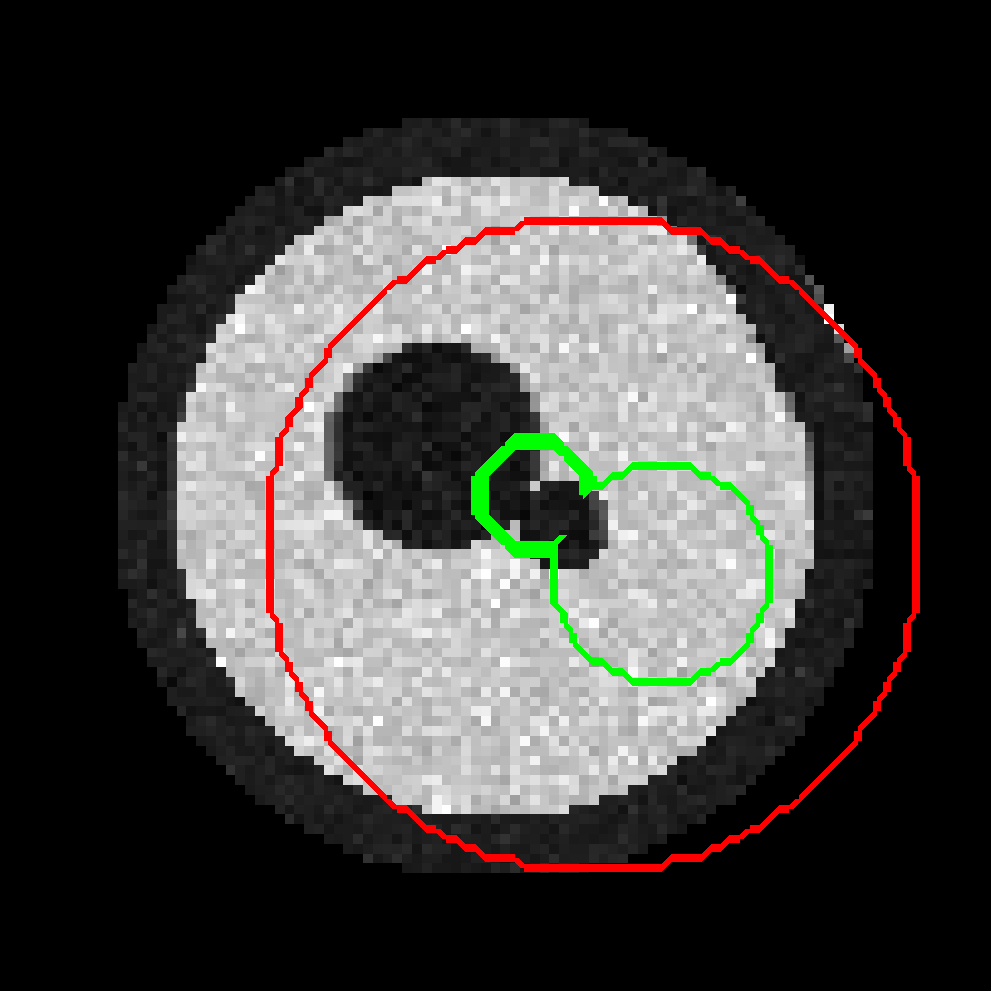
\includegraphics[width=0.19\textwidth]{model1result_b_3} &
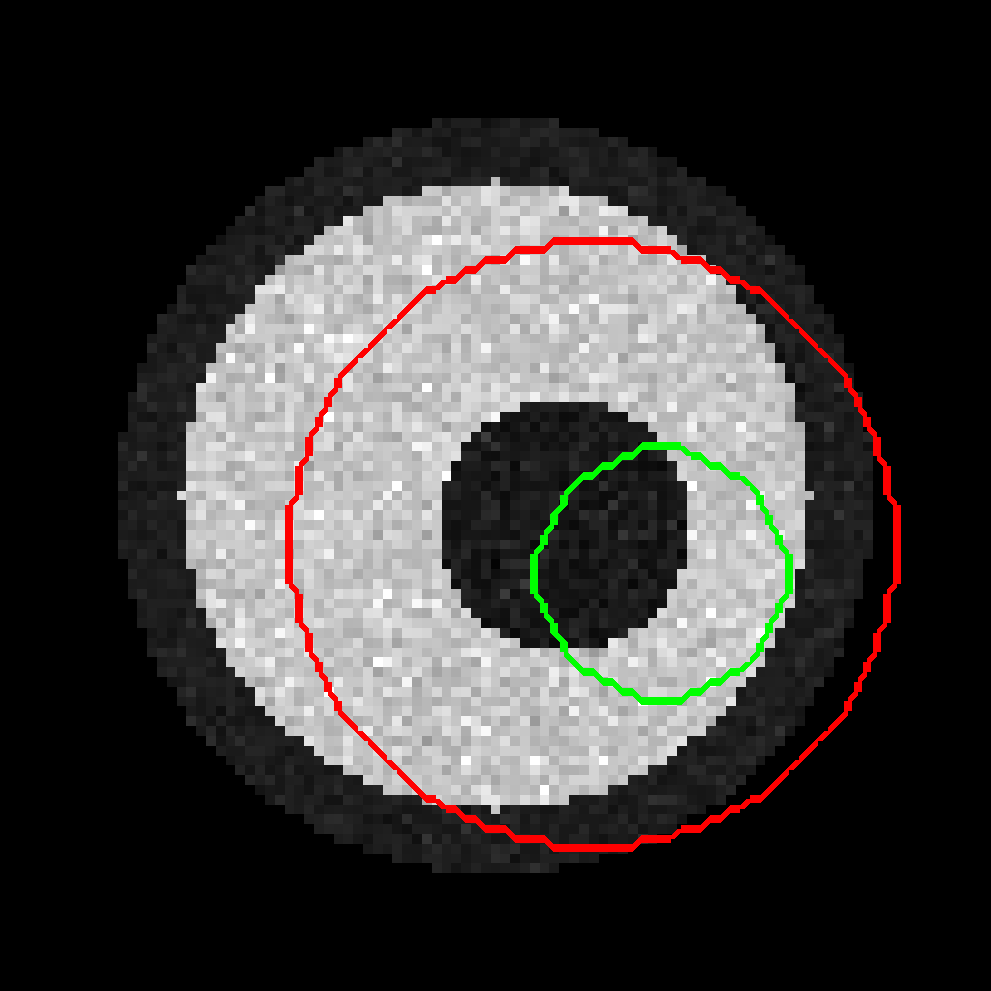
\includegraphics[width=0.19\textwidth]{model1result_b_4} &
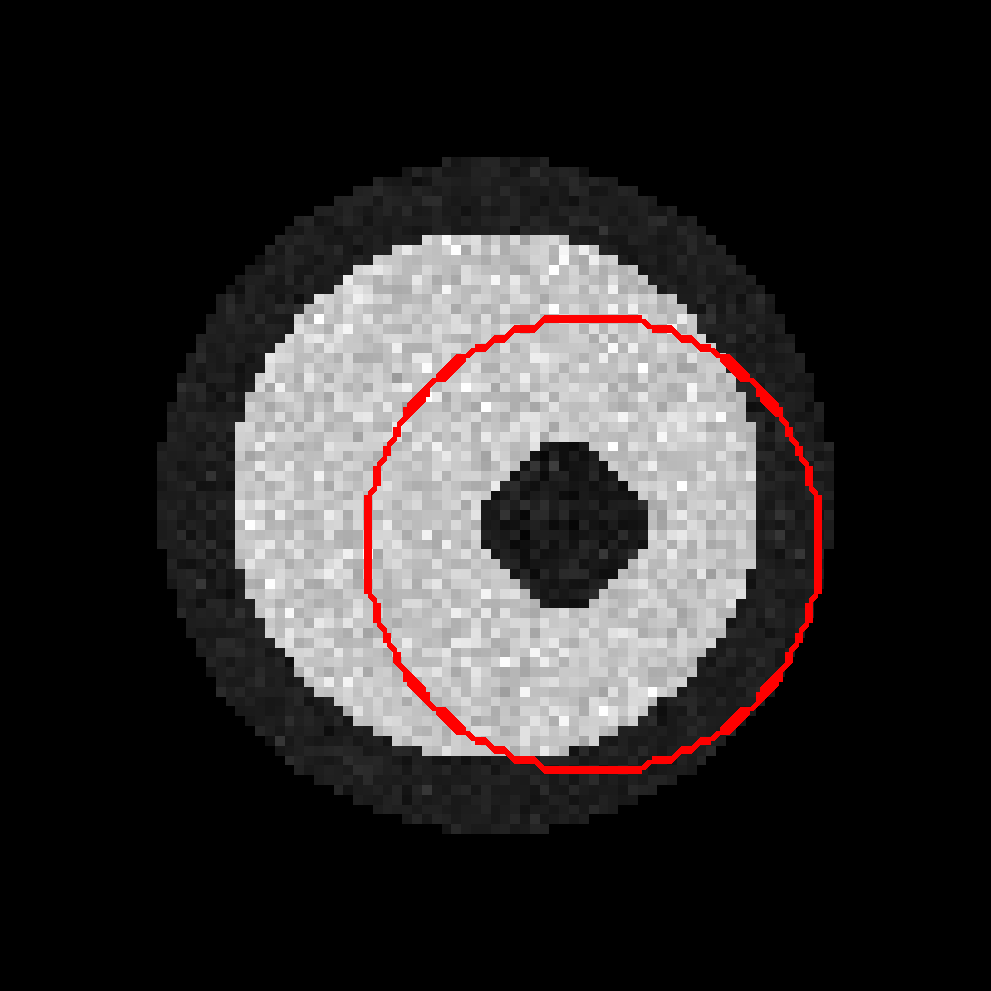
\includegraphics[width=0.19\textwidth]{model1result_b_5} \\
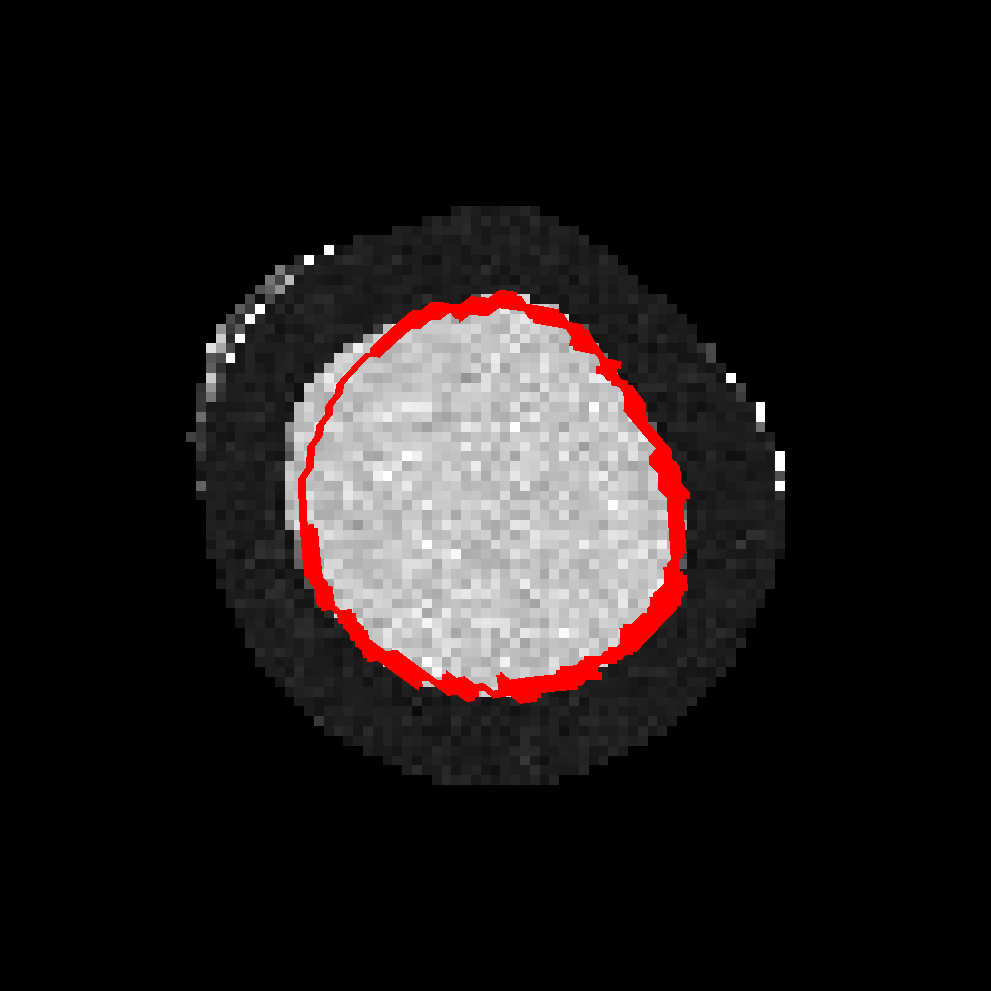
\includegraphics[width=0.19\textwidth]{model1result_a_1} &
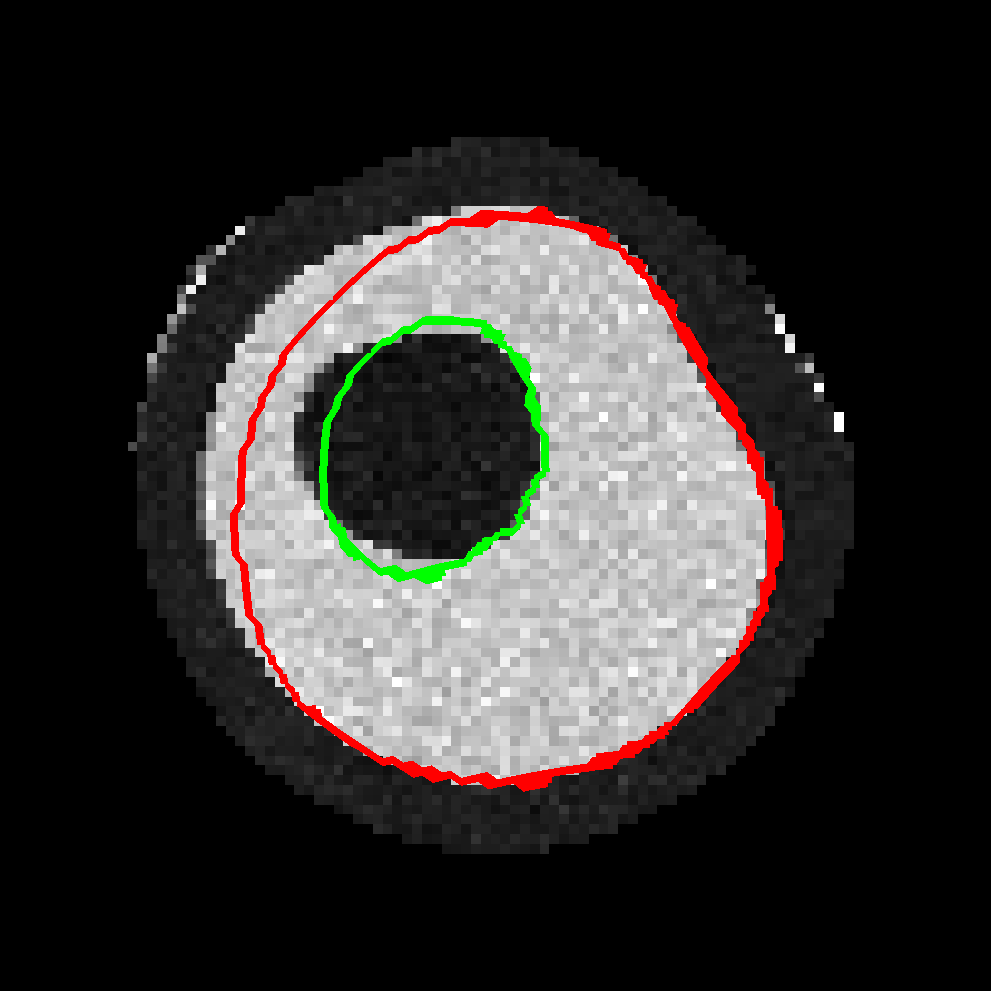
\includegraphics[width=0.19\textwidth]{model1result_a_2} &
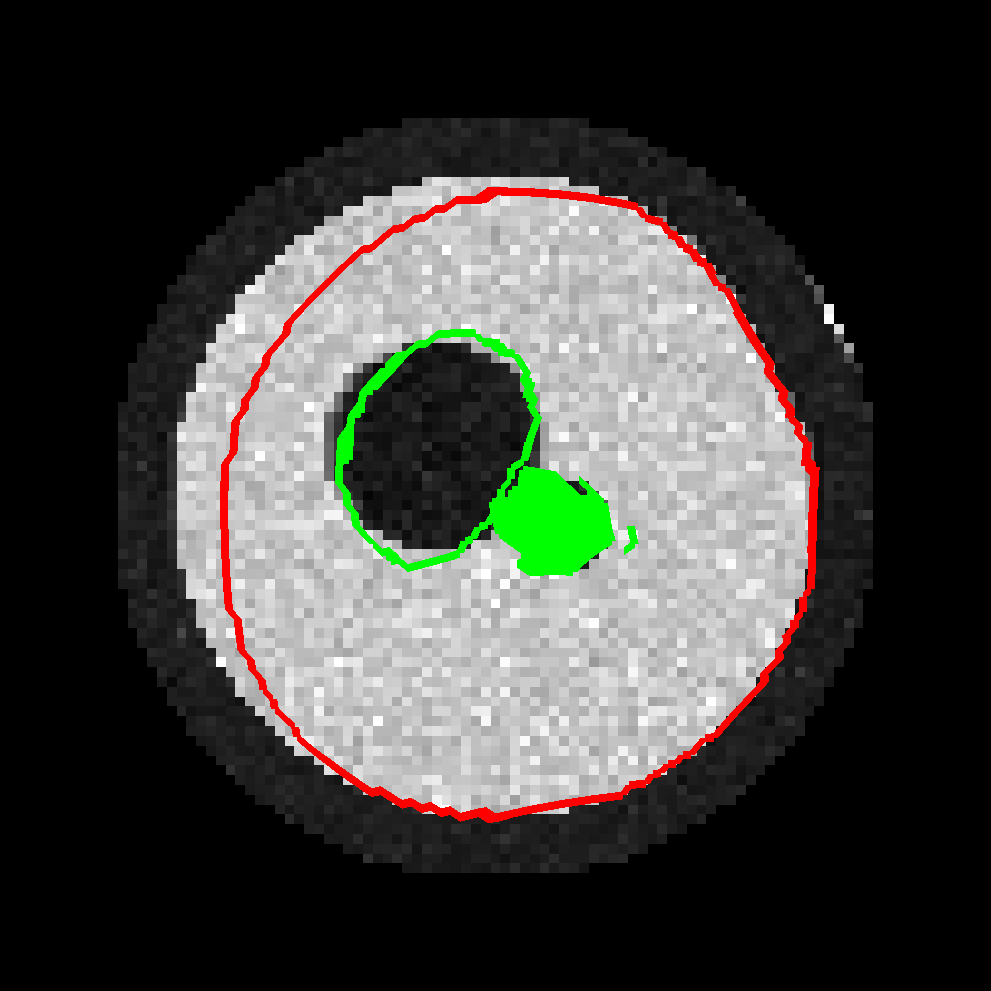
\includegraphics[width=0.19\textwidth]{model1result_a_3} &
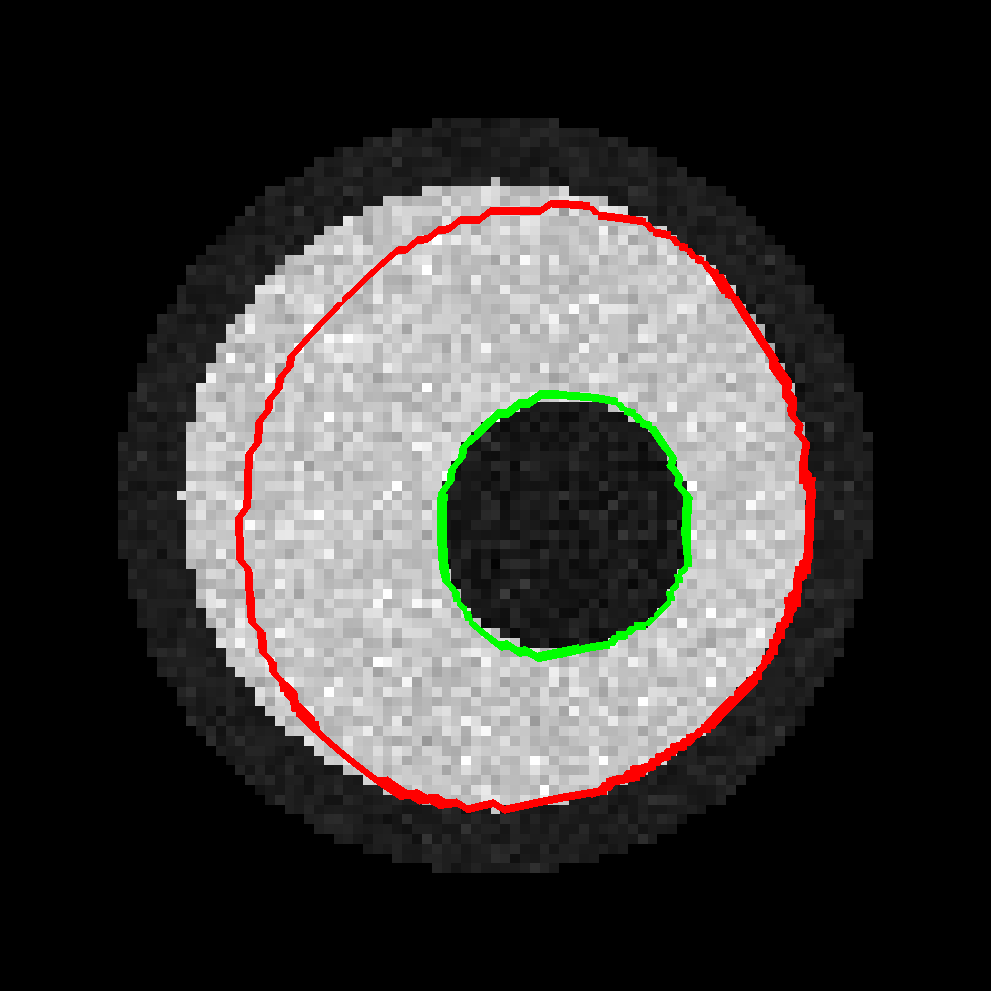
\includegraphics[width=0.19\textwidth]{model1result_a_4} &
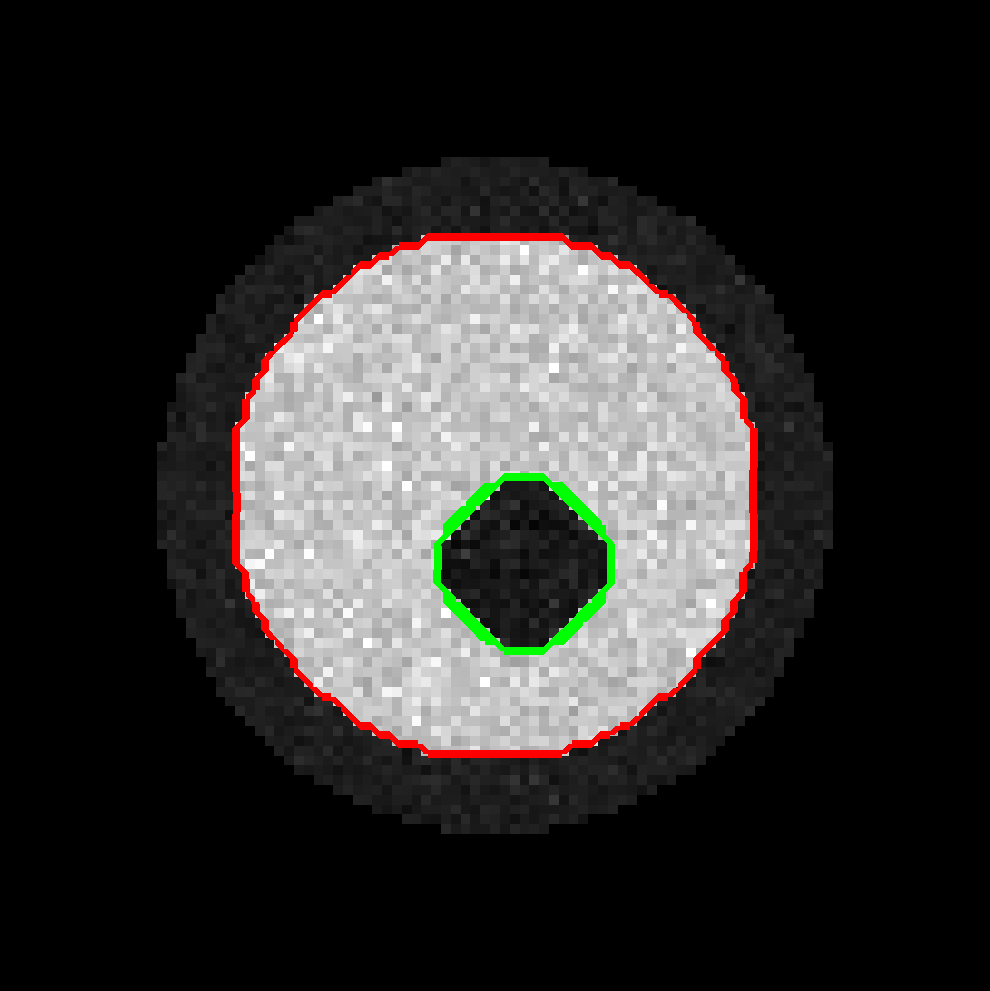
\includegraphics[width=0.19\textwidth]{model1result_a_5} \\
\end{tabular}
\caption{First row presents several slices along Z axis of the distorted \ac{fa} map and
the undistorted \ac{wm}-\ac{gm} and \ac{wm}-\ac{csf} contours given as shape priors. Second row contains the same map, now with the contours after joint segmentation-registration.}
\label{fig:fa}
\end{figure}

\section{Conclusions and outlook}
\label{sec:conclusion}
%
A novel application for the \gls{acwe} framework is proposed,
with the aim at recovering the displacement field underlying 
the \gls{epi} geometrical distortions. Exploiting the segmentation
properties of the \gls{acwe} and optimizing the displacement
field, we describe a registration-segmentation methodology that
simultaneously segmented and restored the distortion on 
\gls{dwi}-like synthetic data. Visual results and quantitative
results are provided. \\

We implemented the methodology upon the widely used
Insight Registration and Segmentation 
Toolkit~\footnote{\url{http://www.itk.org}} (ITK)
for its computational benefits, the standardized code, and 
with the aim at making the procedure publicly available 
when ready for sharing with the research community.

Once proven the aptness of the methodology to the application
with simplistic synthetic data, in further studies we will 
cover the actual performance on real images and the benefits 
of overcoming the described challenges (segmentation and 
\gls{epi} distortion correction) in one single step.\\

We conclude stressing on the importance of tackling with
the numerous challenges that exist on the \gls{dwi} data 
processing in order to achieve reliable results on the
whole-brain connectivity analysis.


\bibliography{99-References}

\end{document}
